

\documentclass{article}

% packages
\usepackage{graphicx} % pictures
\usepackage{listings} % source codes
\usepackage{xcolor} % source codes highlight
\usepackage{threeparttable} % result table
\usepackage[backend = biber, style = caspervector, utf8, sorting = none]{biblatex} % references
\usepackage{geometry}
 \geometry{
 a4paper,
 total={170mm,257mm},
 left=25mm,
 top=25mm,
 right=25mm,
 bottom=25mm
 }




\begin{document}

% format

\setlength{\parskip}{1em}

% titles

\title{CSE 221 Project Report}

\author{Yudong Wu, A53216872\ \texttt{yuw466@eng.ucsd.edu}
        Chengcheng Xiang, A53219708\ \texttt{c4xiang@ucsd.edu}
        Yihong He, A53218157\ \texttt{yih251@eng.ucsd.edu}
}

\maketitle

% lstlisting set
\lstset{
    numbers=left,
    numberstyle=\footnotesize,
    stepnumber=1,
    numbersep=5pt,
    basicstyle=\footnotesize,
    frame=single,
    tabsize=2,
    breaklines=true,
    xleftmargin=2em,
    xrightmargin=2em,
}

% introduction
\section{Introduction}


The goal of this project is to measure the performance characteristics of a HP's workstation in Opera group when running ubuntu 16.04.4. There is 3 people in our group: Chengcheng, Yihong and Yudong. We finished this system measurement project by C, a typical system implementation languages. Our code is compiled by gcc 5.4.0, with optimization flag \textbf{-O0}. 



% machine description
\section{Machine Description}

Our experiment machine is an HP Pavilion Elite HPE workstation, and the system running on this machine is Ubuntu 16.04.1. The specs of this machine and the operating system will be stated below.

\subsection{CPU}

The processor on this machine is an Intel(R) Core(TM) i7 CPU 860 @ 2.80GHz with 4 cores. This CPU supports constant tsc feature, which makes cycle counting much more trivial. When running this project, we disabled 3 of the 4 cores, and made only a single core available for running our measurement benchmark. The specs summery for this core is listed below:

\begin{itemize}
    \item The frequency of this CPU should be 2.80GHz (read from model infomation). After a simple measurement, we found out that the frequency of the clock of this core is 2.793291 GHz, and the clock period of this core should be $$ \frac{1.000000}{2.793291 GHz} = 0.358001 ns $$
    \item This core has 64K on core L1 cache, which 32K of them are data cache, and the rest 32K are instruction cache
    \item This core has 256k on core unify L2 cache
    \item The L3 cache is 8M, and it is shared by all cores. Since we only enable single core when running, we can seem it as a private 8M L3 cache for this core.
    \item For the precision purpose, we turned off multi-threading and turbo boosting feature on this core
\end{itemize}

\subsection{Memory}

This machine has totally 8G main memory, with 4 bank of 1333 MHz DDR3.

\subsection{Buses}

The memory bus is with 64 bits width and 1333 MHz clock. The IO bus is PCI bus with 32 bits width and 33MHz clock.

\subsection{Disk}
The machine has a 750GB SATA hard drive disk. The disk model is HDS721075CLA332 with 32MB cache and 7200RPM spindle speed. The external data transfer rate is 300Mbps.

\subsection{NIC}

The NIC is RTL8111/8168/8411 PCI Express Gigabit Ethernet Controller with 1Gbit/s capacity.

\subsection{Operating System}
When running this project, the operating system running on the machine is normal Ubuntu 16.04.1. The kernel is Linux 4.4.0-57-generic x86\_64.


% experiments
\section{CPU Operations}

This section mainly reports our estimation and measurement result about the cpu operations and os service like system calls and context creation and switch.


\subsection{Overhead Measurement}
When performing measurement, we are using the following code to measure the overhead of a piece of code:

\lstinputlisting[language=C, firstline=4, lastline=15]{../include/proj_timing.h}

In the source code, we use RDTSC and RDTSCP to read out the timestamp counter register on the cpu. CPUID instruction serves as a barrier to ensure only cycles
runs between RDTSC and RDTSCP instructions will be counted. So when we want to measure the overhead of some functions (code pieces), we can just put START\_COUNT
before the target code pieces and STOP\_COUNT after, then we can easily get the cycles ticks during executing the code pieces we want to measure.


\subsubsection{Methodology}
When measuring the overhead of the measurement code we mentioned above, we use the following code snipes to perform the overhead measurement:

\lstinputlisting[language=C, firstline=21, lastline=22]{../CPU/time_ovh.c}

We just measure nothing between two count marcos, so that this measurement will response the overhead of the execution of thos two marcos.

When performing the measurement, we will run the measurement code in a 10000 round loop, then we take the arithmatic mean of the cycles responsed as the final result.

% because this minimal
% cycles results can be an evidence that our cpu can finish running the target code within this minimal cycles ticks, and also, all other greater cycles ticks might imply that
% they are impacted by other infererence like hardware interruption. As a result, this minimal value is the value that most likely producing without any other infererence, so we take
% this minimal value as the measurement result.

\subsubsection{Estimation and results}
\label{overhead_estimation}

The estimation and the measurement result will be list in the following table:

\begin{table}[ht]
  \centering
  \caption{\textbf{Measurement Overhead: Estimation and Experiment Results}}
  \begin{threeparttable}
  \begin{tabular}{cccc}
  \hline
      \textbf{Hardware Overhead} & \textbf{Software Overhead } & \textbf{Total Overhead} & \textbf{Expr. Results} \\
      \textbf{Estimation}       &  \textbf{Estimation}         & \textbf{Estimation}  &     \\
  \hline
  6 (inst) or 44 (cycles) & 0 & 6 (instructions) & 102 \\
  \hline
  \end{tabular}
  \end{threeparttable}
  \label{measurement_overhead_table}
\end{table}

When estimation, the first evidence for us to perform the estimation is the code we write and generate, following is the acutall assembly code after compilation:

\begin{lstlisting}
    4005f8:	0f a2                	cpuid
    4005fa:	0f 31                	rdtsc
    4005fc:	89 d7                	mov    %edx,%edi
    4005fe:	89 c6                	mov    %eax,%esi
    400600:	89 7d d0             	mov    %edi,-0x30(%rbp)
    400603:	89 75 d4             	mov    %esi,-0x2c(%rbp)
    400606:	0f 01 f9             	rdtscp
    400609:	89 d7                	mov    %edx,%edi
    40060b:	89 c6                	mov    %eax,%esi
    40060d:	0f a2                	cpuid
    40060f:	89 7d d8             	mov    %edi,-0x28(%rbp)
    400612:	89 75 dc             	mov    %esi,-0x24(%rbp)
\end{lstlisting}

We can found out: there are 4 instructions between RDTSC and RDTSCP instruction: two of them are inline aseembly we write in code, and the rest two are compile-time generated code caused by
register saving, so the totally overhead for the measurement should be 4 instructions + 2 instructions (RDTSC and RDTSCP themselves).

The second issue for estimating the hardware overhead is that, how many cycles each instruction will take, or in other words, what is the cpu's CPI (cycles per instruction). We haven't found out
the most related information, so we performed the following estimation: for those 6 instructions, we assume that each cycle the cpu can commit one instruction, and the pipeline stages is around 20;
as those 6 instructions don't have any data dependencies that can not be solved by data forwarding, the pipeline will not stall,and for those 6 instructions, from first instruction enter the pipeline
to the last instruction commit, the cycles consumed should be:
    $$ 20 + 4 + 20 = 44 cycles $$

After the experiments, the result shows that we underestimated the overhead by around 50\%, but as we don't know much about the internal of the Intel CPU, so that this kind of mistakes is somewhat reasonable.

\subsection{Loop Overhead}
When performing estimation, it is reasonable that using repeated experiments to reduce the impact of variance, so before all other overhead measurement, we need to determin the overhead of the loop first.

\subsubsection{Methodology}

When measuring the loop overhead, we simply measures the cycles diff before and after a simple do nothing loop. In order to reduce the impact of variance, we also run this test 10000 times, and then take the arithmatic
means of 10000 samples. We also subtract the time measurement overhead (102 cycles as \textbf{Section \ref{overhead_estimation}}) from the loop overhead, so the final loop overhead should be:
    $$ average(cycles) - 102 $$

We also perform our measurement upon loops rounds from 0 to 50, in order to see the overhead of different loop scale.

\subsubsection{Estimation and results}

Our Estimation and the measurement results are shown in the \textbf{Figure \ref{loop_overhead_result}}:

\begin{figure}[ht]
    \centering
    \frame{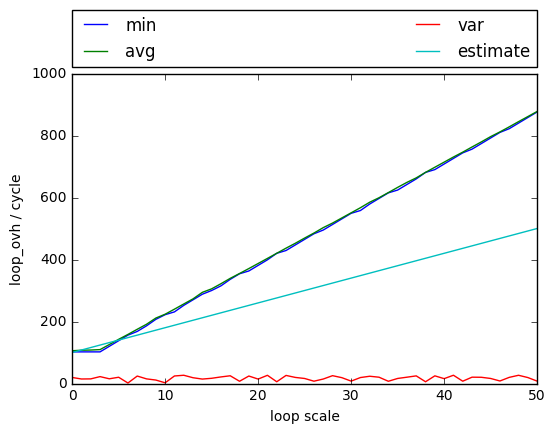
\includegraphics[width = .9\textwidth]{pictures/loop_ovh.png}}
    \caption{Loop Overhead: Estimation and Experiment Results }
    \label{loop_overhead_result}
\end{figure}

As shown in the graph, when estimating, we estimate the overhead increasing by 8 cycles when loop scale increase by 1. We made this estimate based on the instructions of the loop after compile:

\begin{lstlisting}
    4006a1:	c7 45 c4 00 00 00 00 	movl   $0x0,-0x3c(%rbp)
    4006a8:	eb 04                	jmp    4006ae <main+0xf8>
    4006aa:	83 45 c4 01          	addl   $0x1,-0x3c(%rbp)
    4006ae:	8b 45 c4             	mov    -0x3c(%rbp),%eax
    4006b1:	3b 45 c0             	cmp    -0x40(%rbp),%eax
    4006b4:	7c f4                	jl     4006aa <main+0xf4>
\end{lstlisting}

As shown in above, there will be 4 instructions for each round of the loop, as the \textbf{Section \ref{overhead_estimation}} shows that, each instruction will taken more than one cycle tick in average.
We finally made a assumption that each instructions will take up 2 cycles on average.

The result shows that we still underestimated the increament ratio of the overhead, and in fact, each each loop round increase will increase the overhead by 18. The red line is the variance of our data, which shows our result is quite stable.

\subsection{Procedure Call}

\subsubsection{Methodology}

Since procedure call is very quick (our rough measurement shows it takes less than 10 cycles), we measure procedure calls in loops rather than individually to reduce the variance of the measurement's own overhead. The code is as following:

\begin{lstlisting}
for (i = 0; i < outerloop; i++) {
    START_COUNT();
    for (j=0; j < innerloop; j++){
        procedure_0();
    }
    STOP_COUNT();
}
\end{lstlisting}

When calculating the time consumed by procedure\_0, we first calculate the arithmatic mean of the duration cycles collected by START\_COUNT and STOP\_COUNT, then subtract the overhead of the time measurement and the innerloop from it, and finally divide the result by the innerloop times. We set outerloop and innerloop to be 10000 and 50 separately.

%When measuring the overhead of a procedure call, we just put our cycles counting code before and after the procedure call; also, we reduced the variance by using the arithmatic mean of the response overhead came from 10000 times measurements.

\subsubsection{Estimation and results}
We estimate the procedure call with no parameters will take 4 cycles and expect for two additional cycles for every one more parameter.

\textbf{Figure \ref{procedure_overhead_result}} shows our Estimation and the measurement results. The comparison indicates that procedure call is far more quicker than we expected and the overhead increases linearly when the parameter number increases. The variance line justifies that we have successfully eliminated most variance.


\begin{figure}[h]
    \centering
    \frame{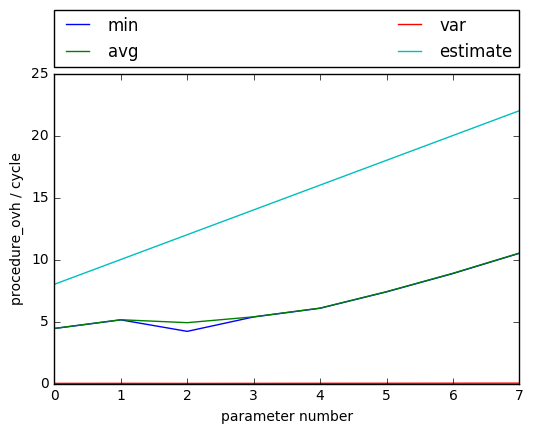
\includegraphics[width = .9\textwidth]{pictures/procedure.png}}
    \caption{Procedure Overhead: Estimation and Experiment Results }
    \label{procedure_overhead_result}
\end{figure}


\subsection{System Call}

\subsubsection{Methodology}

When measuring the system calls, basically we want to measure the cycle ticks between the begin and the return points of the system call. This means that we require the kernel return the control to the process immediately after the system call service routine finishes, so that what we can measure is some 'light weight' system call, like \textbf{getpid()} or \textbf{getcwd()}. However, \textbf{getpid()} will be cached by the kernel, so that only the first call of the getpid() can trap into
the kernel space, so that in the end, we choose \textbf{getcwd()} system call to be the system call we measured.

For specific implementation, the measurement process will first start counting cycles, then invoke \textbf{getcwd()} system call, finally stop counting. The cycles counted should be the overhead of the \textbf{getcwd()} system call.


\subsubsection{Estimation and results}

The estimation and the measurement results are shown in \textbf{Table \ref{measurement_syscall_table}}

\begin{table}[ht]
  \centering
  \caption{\textbf{System Call Overhead: Estimation and Experiment Results}}
  \begin{threeparttable}
  \begin{tabular}{ccccc}
  \hline
      \textbf{Hardware Overhead} & \textbf{Software Overhead } & \textbf{Total Overhead} & \textbf{Expr. Results} & \textbf{Standard}\\
      \textbf{Estimation}       &  \textbf{Estimation}         & \textbf{Estimation}  &     & \textbf{Deviation}\\
  \hline
  1000 inst & 0 & 1000 inst & 1250 & 31 \\
  \hline
  \end{tabular}
  \end{threeparttable}
  \label{measurement_syscall_table}
\end{table}

For estimation, system calls in a 64-bit system will first save a bunch of system call parameters into registers, then trap into the kernel by invoke \textbf{int} instruction or \textbf{syscall} instruction, then the kernel will serve the system call, and finally turn back to user mode with similar cost with trap into the memory. As there is a lot of assistance routine when traping into the system, then we believe 1000 cycle shoule be a reasonable estimation.

The results shows that our estimation is quite accurate.

For the questions about comparison between system call and procedure call, system call is definitely much heavy weight than procedure call, as a procedure call with 7 parameters only cost 11 cycles, but the system call will cost more than 1000 cycles. This is caused by a lot of checking and setting operations when traping into kernel mode and return to user mode.

\subsection{Process and Kernel Thread Creation}

\subsubsection{Methodology}
\label {creation_methodology}

When measuring Task, or process creation time, we need to ensure serveral things. The first one when the measurement process fork a child process after fork syscall, the os will schedule either the measurement process or the child of the measurement process to be executed. To ensure that, we run our measurement process with the round robin real time schedualer and set the process the highest priority. The cmd is as follows:

\begin{lstlisting}
    sudo chrt -rr 99 ./measurement
\end{lstlisting}

However, even we make our process the highest priority,  we are still not sure which process (parent, or child) will be executed first. So we need to ensure to handle both cases so that we can get the cycles between the point just before fork call and the point fork return.

In order to get the results we want, we implement the following measurement sequence:

\begin{enumerate}
    \item We initialize a pipe for child and parent process to comunicate \label{task_creation_pipe}
    \item We start counting cycles before we call fork
    \item Both at the parent and the child process start point after fork return, we stop counting cycles
    \item Child process passing the end counting to the parent via the pipe we initialized at \textbf{\ref{task_creation_pipe}}
    \item We calculate both cycles spend for parent fork return and child fork return, then choose the smaller one (as the smaller one indicates that this process executes before the other one)
\end{enumerate}

For the kernel thread creation, we use a similar method. The measurement sequence is listed at following:
\begin{enumerate}
    \item We initialize a global variable for child process to store the end clock cycle count \label{thread_creation_gv}
    \item We start counting cycles before we call pthread\_create
    \item Both at the main and the peer thread start point after pthread\_create finished, we stop counting cycles
    \item peer thread passing the end counting to the main thread via the global variable we initialized at \textbf{\ref{thread_creation_gv}}
    \item We calculate both cycles spend for main thread pthread\_create return and pthread\_create start execution, then choose the smaller one (as the smaller one indicates that this thread executes before the other one)
\end{enumerate}

We repeate each measurement for 10000 times to get the accurate cycles.

\subsubsection{Estimation and results}

The estimation and the measurement result will be list in the \textbf{Table \ref{process_creation_time}}:

\begin{table}[ht]
  \centering
  \caption{\textbf{Process/Thread Creation Time: Estimation and Experiment Results}}
  \begin{threeparttable}
  \begin{tabular}{cccccc}
  \hline
      \textbf{Process or} & \textbf{HW Overhead} & \textbf{SW Overhead } & \textbf{Total Overhead} & \textbf{Expr. Results} & \textbf{Standard}\\
      \textbf{Kthread} & \textbf{Estimation}       &  \textbf{Estimation}         & \textbf{Estimation}  & (AVG)   & \textbf{Deviation} \\
  \hline
      \textbf{Process} & NA & NA & 20000 ($7.16 \mu s$) & 134507 & 3062 \\
      \textbf{Kernel Thread} & NA & NA & 10000 ($3.58 \mu s$) & 20635 & 1546 \\
  \hline
  \end{tabular}
  \end{threeparttable}
  \label{process_creation_time}
\end{table}

When we make estimation, it is hard for us to do the hard ware and software estimation, as there are a lot of issues hard to estimate. For example, for fork(), the kernel will create a new process control block for the new process, and then set
up a bunch of member's value inside the pcb; after that, it will at least initialize the child process's address space, by creating a bunch of page tables; all these operations might cost more then 20000 cycles. Compared with process creation,
thread creation is much more light weight, as thread doesn't need to construt a new address space. Finnally we made a pridiction that, process creation will cost 20000 cycles and thread will cost half of the process cost, 10000 cycles; or in other
word, $7.16 \mu s$ for process and $3.58 \mu s$ for thread.

Our experimental results show that the process creation and thread creation takes 134507 and 20635 cycles correspondingly, which means creating a process takes much longer time than we have estimated and creating a thread is much more lightweight. The standard deviations for our experiments are 3062 and 1546, which are relatively small to the average results.


\subsection{Process and Kernel Thread Context Switch}

\subsubsection{Methodology}

For the overhead measurement of the context switch, the basic idea to measure the overhead is to count the cycles spend on switch from one process (thread) to another process (thread). To make our measurement accurate, we need to ensure the same thing we indicates in
\textbf{section \ref{creation_methodology}}, that the measuring processes (threads) are the only two processes (threads) that to be scheduled. In the real system, this is impossible, but we can estimate this situation by increasing the priority of the process (threads).

For specific how to count the cycles of a context switch, we need to force a context switch to happen in one process (thread) the another (thread) process can stop the counting afterwards. To achieve this goal, we implement the following measure sequence by using blocking
reading pipe. To be more precisely, at parent process, we first start a pipe for communication, then fork new process; after that, parent process will first start counting cycles, then write to the communiting pipe, then call wait() to wait the child process; at the same time, child process will read from the pipe, then stop counting the cycles, and finally send the stop cycles back to the parent process via the pipe then exit; after that, parent will wake up and get the value and count the tick.

This method uses read and wait to synchronize. Either child or parent process executing first, the final result will be the period start from parent writing to the pipe, then context switch to the child, and finally the the child read from pipe.

The method for thread is similar, the differences are:

\begin{enumerate}
    \item We use pthread\_join() instread of wait()
    \item We use global variable, instead of pipe, to pass the final tick to the main thread;
\end{enumerate}


\subsubsection{Estimation and results}
\begin{table}[ht]
    \centering
    \caption{\textbf{Process/Thread Context Switch Time: Estimation and Experiment Results}}
    \begin{threeparttable}
        \begin{tabular}{cccccc}
        \hline
        \textbf{Process or} & \textbf{HW Overhead} & \textbf{SW Overhead } & \textbf{Total Overhead} & \textbf{Expr.        Results} & \textbf{Standard} \\
        \textbf{Kthread} & \textbf{Estimation}       &  \textbf{Estimation}         & \textbf{Estimation}  & (AVG)   & \textbf{Deviation}\\
        \hline
        \textbf{Process} & NA & NA & 20000 & 79097  &  650\\
        \textbf{Kernel Thread} & NA & NA & 10000 & 2562 & 538\\
        \hline
        \end{tabular}
    \end{threeparttable}
    \label{context_switch_time}
\end{table}

For the estimation of the overhead of a context switch, we are not pretty sure the precise overhead of the context switch, so we just make a guess that the overhead should be more then 10000 cycles for thread, and the overhead for the process should be at least twice as the thread's.

The final results shows that we under estimate the overhead of the process context switch, and it should be around 80000 cycles; but amazingly for the thread one, it only cost around 2500 cycles for context switch. We might perform some more measurement about that in the future.

For the question about difference between process context switch and kernel context switch, as the results show that, the overhead of thread context switch around 30 times less then process context switch. The main difference between thread and process context switch
is that, when thread context switching, kernel need neither to construct the virtual memory space to the thread switch to, nor to flush the tlb, which means that thread context switch is much less expensive than process context switch.


\section{Memory}

% \addbibresource{./references.bib}

This section we will mainly discuss our measurement about memory performance on the target machine. More specifically, we will report measurements about access latency on each level of memory hierarchy, the memory bandwidth, and the overhead of page fault handling.

\subsection{Memory Latency}

\subsubsection{Methodology}

When measuring access latency on each level of memory hierarchy, basically we followed the method suggest by lmbench\cite{mcvoy1996lmbench}.

We create a linklist which only contains a pointer to the next element:

\begin{lstlisting}
    struct Linklist {
        struct Linklist * next;
    };

    typedef struct Linklist Linklist;
\end{lstlisting}

The total size of the linklist will increase from 1 KB to 256 MB, by the factor of 2. When initializing, a stride will be provided by the tester. The number of the elements in the linklist is always divisible by the stride, and when initializing, the linklist will be decided as many chunks contains stride elements, and each elements in one chunk will point to a random element in the next chunk, and the last chunk in the linklist element array will point to the first chunk, which make this linklist an infinite cyclical linklist. This structure will eliminate the impact of cache prefetch, as the stride and random elements can easily make the next element in the linklist out of the prefetch range of each level of cache.

When performing measurement, in order to get rid of all other unnecessary memory access, we have to use at least \textbf{O1} optimization; however, \textbf{O1} optimization will also optimized the code accessing the linklist. In our final measurement code, the travel of the linklist if write in inline assembly which can avoid compiler optimizations:

\begin{lstlisting}[language=C]
    START_COUNT(high, low);
    while (step --> 0) {
#define INST "movq	(%%rax), %%rax\n\t"
        asm volatile ("mov %0, %%rax\n\t" \
                       HUNDRED(INST) \
                       "mov %%rax, %1"
                       : "=r" (iter)
                       : "r" (iter)
                       : "%rax");
    }
    STOP_COUNT(high1, low1);
\end{lstlisting}

where iter is the head of the linklist. We will measure 100 times of accessing memory on each measurement, and totally perform 1000 (stored in \textbf{step}) measurements.

\subsubsection{Estimation and Results}

\begin{figure}[ht]
    \centering
    \frame{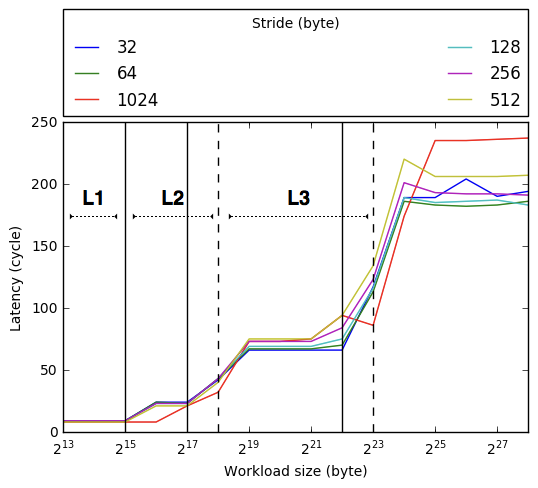
\includegraphics[width = .9\textwidth]{pictures/memLatency.png}}
    \caption{Memory Hirachy Latency: Estimation and Experiment Results }
    \label{mem_latency_result}
\end{figure}

\begin{table}[ht]
  \centering
  \caption{\textbf{Memory hierarchy Latency: Estimation and Experiment Results}}
  \begin{threeparttable}
  \begin{tabular}{ccc}
  \hline
      \textbf{Memory}    & \textbf{Latency}   & \textbf{Expr. Results} \\
      \textbf{Hiracht}   & \textbf{Estimation}  & (AVG)   \\
  \hline
      \textbf{L1}  & 5 cycles (1.79 ns) & 9 cycles (3.22 ns)   \\
      \textbf{L2}  & 20 cycles (7.16 ns) & 20 cycles (7.16 ns)  \\
      \textbf{L3}  & 60 cycles (21.48 ns) & 70 cycles (25.06 ns)  \\
      \textbf{Memory}  & 150 cycles (53.70 ns)  & 190 cycles (68.02 ns)  \\
  \hline
  \end{tabular}
  \end{threeparttable}
  \label{memory_latency_table}
\end{table}

For estimation, we believe the latency for l1 cache references should be pretty low, let's say, within 5 cycles; the latency for l2 cache should be higher, let's say, 20 cycles; the latency for l3 cache should be much higher than l2, let's say, 60 cycles; and the latency for main memory should be the highest and much higher than l3 cache, let's say, 150 cycles.

The result is shown in \textbf{Figure \ref{mem_latency_result}} and \textbf{Table \ref{memory_latency_table}}. In \textbf{Figure \ref{mem_latency_result}}, the real lines separate the latency turning point for different level of memory hierarchy, and the dotted lines separate the real size of different level of memory hierarchy in the target machine. As we can see in the figure, the dotted line and the real line for l1 cache is on the same position, but for l2 cache and l3 cache, the latency turning point is always a little bit smaller than the actual size point. For why that happened, we guess that the following reason contribute it: as both l2 and l3 cache are unify instruction and data cache, so that some instructions stored in the l2 cache and l3 cache will accelarate that data access latency turning point to happen.

\textbf{Table \ref{memory_latency_table}} shows the latency estimation and measurement results. We under estimate the access latency of l1 cache and memory.

\subsection{Memory Bandwidth}

\subsubsection{Methodology}

When measuring memory bandwidth, we use the method metioned in \cite{mcvoy1996lmbench}, which is using integer reading and writing which miss at l3 cache to measure the reading and writing bandwidth for main memory. However, there are several technical details not mentioned in \cite{mcvoy1996lmbench} we need to point out here.

First, although we are reading and writing 4 Byte integers when measuring code, when calculating memory bandwidth, we need to use 64 Byte as the size for each memory access, as when transfering data back and forth between main memory and l3 cache, data is always transferred with a l3 cache line size. The l3 cache line size can be retrieve by command:

\begin{lstlisting}
    cat /sys/devices/system/cpu/cpu0/cache/index3/coherency_line_size
\end{lstlisting}

At the same time, in order to get ride of cache line prefetch, we need to accesing data with a stride at least as large as the l3 cache line size. In our experiments, we use 256 byte (or 64 integers) as a accesing stride.

Furthermore, by using command:

\begin{lstlisting}
    sudo lshw -C memory
\end{lstlisting}

we can retrive the writing policies for each level cache. In our experiment computer, l1 and l2 cache are both write-through cache, while l3 cache is a internal write-back unified cache. Although it does not mention the write miss policy, \cite{wiki:cache} indicates that write back policy usually pairs with write allocation policy. Due to these fact, there is some details in the implementation:

\begin{enumerate}
    \item In order to get ride of caching effect of l3 cache, we first fill l3 cache with data that will never be read and write during measurement process.
    \item When measuring reading bandwidth, we need to fill l3 cache with clean cache lines, orderwise when we reading the measurement data from main memory to l3 cache, there will be a high dirty block writing back overhead when evict cache lines.
    \item When measuring writing bandwidth, we want all measurement data to experience a write miss. However, l3 cache itself is write allocation, thus even a write miss will not write back to main memory. In this case, the way we solve this problem is filling all l3 cache line with dirty cache data before we start measurement. As a result, each time we write a measurement writing data, as l3 cache is a write allocation cache with full of dirty data, so that each time l3 cache will evict a dirty line as each time we are accessing different l3 cache set, which means that each time we write, we will finally write a dirty cache line back to main memory, and thus we can measure the memory writing bandwidth.
\end{enumerate}

\subsubsection{Estimation and Results}
\label{Memory_bandwidth_result_section}

\begin{table}[ht]
  \centering
  \caption{\textbf{Memory Bandwidth: Estimation and Experiment Results}}
  \begin{threeparttable}
  \begin{tabular}{ccccc}
  \hline
      \textbf{Read or} & \textbf{Bandwidth}   & \textbf{Expr. Results} & \textbf{Standard}\\
      \textbf{Write}   & \textbf{Estimation}  & (AVG)   & \textbf{Deviation} \\
  \hline
      \textbf{Read}  & 10600 MB/s & 7131.15239595 MB/s & 394.490122927  \\
      \textbf{Write} & 10600 MB/s & 6709.49876645 MB/s & 1191.12060254  \\
  \hline
  \end{tabular}
  \end{threeparttable}
  \label{memory_bandwidth_table}
\end{table}

For estimation, Frank Denneman stated on his web blog \cite{frankdenneman} that, the bandwidth for both reading and writing of a DDR3-1333 memory is 10600 MB/s, we take this as our estimation.

The measurement result is shown in \textbf{Table \ref{memory_bandwidth_table}}. The results shows that memory reading bandwidth should be \textbf{7131.15239595 MB/s}, and writing bandwidth should be \textbf{6709.49876645 MB/s}. Measurement result is below the estimation value, we think the reason for that is:

First, in this experiments, under our accessing pattern, it is hard for main memory to achieve its theorical optimized reading and writing speed, as the bank row cache inside the DRAM will miss, thus an entire row and column retrive process is needed each time we accessing;

Second, the software overhead is unavoidable, this will also decrease our memory performance.

The writing bandwidth is smaller than reading bandwidth, as \textbf{Table \ref{memory_bandwidth_table}} shown. This is reasonable, as writing do be slower than reading in DRAM.

\subsection{Page Fault Handling}

\subsubsection{Methodology}

When measuring page fault handling overhead, we will first create a large file (40 MB) on disk, then using \textbf{mmap()} system call, to map the file into the main memory. Then, we will reading data in that file, as \textbf{mmap()} only mapping that file into destination memory chunks, not reading file contents into main memory, the reading operation will cause a page fault. The operating system will handle that page fault, and that's what we want to measure.

There is still one problem needs to be addressed out, the file system optimization. The file system will cache the contents of the file and also perform file prefetch from the disk, so that, if we failed to bypass those optimization, we could not accurately measure the page fault handling overhead. To bypass those optimization, the measurement program will access the file with a stride applied with a random offset on page.

We used to create a 150 MB file in /tmp directory for mapping, however, it turns out that the overhead for handling pagefault after mapping in this file is significantly smaller than a HDD's overhead, and there is no seek penalty exist, and obviously this file is actually stored in memory. In the second round, we changed the directory for the tmp mapping file to the current directory of the benchmark binary, the expanded the file size to 16 GB, after that, we can observe seek penalty now.

\subsubsection{Estimation and Results}

\begin{table}[ht]
  \centering
  \caption{\textbf{Pagefault Handling Overhead: Estimation and Experiment Results}}
  \begin{threeparttable}
  \begin{tabular}{cccccc}
  \hline
        \textbf{HW Overhead} & \textbf{SW Overhead } & \textbf{Total Overhead} & \textbf{Expr. Results} & \textbf{Standard}\\
        \textbf{Estimation}       &  \textbf{Estimation}         & \textbf{Estimation}  & (AVG)   & \textbf{Deviation} \\
  \hline
        28000000 cycles & 10000 cycles & 28010000 cycles (10.03 ms)  & 22672005.8858 cycles (8.12 ms) & 7299383.2799 \\
  \hline
  \end{tabular}
  \end{threeparttable}
  \label{pagefault_handle_time}
\end{table}

For estimation, the I/O speed of a 7200 RPM HDD is at the scale of 100 MB/s \cite{wiki:hdd}, so that transferring a 4K page will take:

$$ \frac{4KB}{100 MB/s} = \frac{1}{25600} s $$

$\frac{1}{25600} s$ equals to around $111600 cycles$.

In checkpoint 2 we made a mistake: we ignored that in a HDD environment, seek and rotation is the most significant overhead for page fault handling, when taking in consider about seek and rotation, the time consumption is of the order of 10 ms. So that, the hardware overhead should be:

$$\frac{10 ms}{0.350001 ns/cycle} = 27932882 cycles$$

So the totally hardware overhead should be around $28000000 cycles$

The software overhead mainly comes from page table maintains and protection mechanism, and we assume this overhead is around 10000 cycles. Then, the total estimation overhead for a pagefault handling is 28010000 cycles.

The result is shown in \textbf{Table \ref{pagefault_handle_time}}. We underestimate the overhead of the pagefault handling by around 2 ms. As there is a high variance for the performance of the disk, it is not strange that this difference exist. It will not experience the largest disk access overhead for each access request.

The result is shown in \textbf{Table \ref{pagefault_handle_time}}. The speed is a little bit faster than what we estimate, this should be caused by each time a page fault happened, the disk seeking and rotation overhead is not always as high as 10 ms.

For the question about speed compare between memory bandwidth and page fault page transfer bandwidth on byte scale, according to \textbf{Section \ref{Memory_bandwidth_result_section}}, on average the memory can transfer a byte in

$$\frac{1 Byte}{7131.15239595 MB/s} = 0.133734 ns $$

and the page fault mechanism can transfer a byte in

$$\frac{1 Byte}{\frac{4 KB}{8.12 ms}} = 1982.421875 ns $$.

Thus the page fault handling is around 15000X more expensive than a page hit memory access.


\section{Networking}

% \addbibresource{./references.bib}

This section we will mainly discuss our measurement about network performance on the target machine. More specifically, we will report measurements about round trip time, peak bandwidth and connection overhead for the TCP protocol.

\subsection{Machine Description}
\label{Network_machine_desc}
In our experiments of this part, the client is running on the original machine and the server is running on the new machine. Below is the machine description of the server.

\subsubsection{CPU}

The processor on this machine is an AMD Athlon(tm) II X4 630 Processor @ 2.80GHz with one core.

\subsubsection{Memory}

This machine has totally 4G main memory.

\subsubsection{NIC}

The NIC is Broadcom Corporation NetLink BCM57788 Gigabit Ethernet PCIe with 1Gbit/s capacity.

\subsubsection{Disk}
The machine has a 160GB SATA hard drive disk. The disk model is ST3160812AS with 8MB cache and 7200RPM spindle speed. The external data transfer rate is 300Mbps.

\subsubsection{Operating System}
When running this project, the operating system running on the machine is normal Ubuntu 16.04.1. The kernel is Linux 4.4.0-51-generic x86\_64.

\subsection{Round Trip Time}
\label{Network_rtt}
\subsubsection{Methodology}

When measuring round trip time, basically we measure the round trip time by calculating time interval between the send time and the ack time for each packet. We first start a TCP server and a TCP client. And then, the client connects the server and sends one byte data to the server every 1 millisecond. We use tcpdump to capture TCP traffics on the client side and calculate the round trip time according to the tcpdump result.  We recognize the send and the ack packet by checking whether two consecutive packets match the flag patterns [P.] and [.] respectively. Below is an example of the send and ack pattern for remote interface:

\begin{lstlisting}
23:10:17.953051 IP 0xcc.ucsd.edu.39660 > dyn54.sysnet.ucsd.edu.9014: Flags [P.], seq 1:2, ack 1, win 229, options [nop,nop,TS val 890347228 ecr 200781447], length 1
23:10:17.953387 IP dyn54.sysnet.ucsd.edu.9014 > 0xcc.ucsd.edu.39660: Flags [.], ack 2, win 227, options [nop,nop,TS val 200781447 ecr 890347228], length 0
\end{lstlisting}

In order to make the round trip time more accurate, on the server side, we mark each socket quick ack, which means that the TCP server immediately reply an ack after receiving each packet. In our experiment, the TCP client sends 10,000 times 1 byte data to the server.

\subsubsection{Estimation and Results}

\begin{table}[ht]
  \centering
  \caption{\textbf{Round Trip Time: Estimation and Experiment Results}}
  \begin{threeparttable}
  \begin{tabular}{ccccc}
  \hline
      \textbf{Remote or} & \textbf{RTT}   & \textbf{Expr. Results} & \textbf{Standard}\\
      \textbf{Local}   &  \textbf{Estimation}  & (AVG)   & \textbf{Deviation} \\
  \hline
      \textbf{Remote}  & 0.395ms & 0.338 ms & 0.099 \\
      \textbf{Local} & 0.025ms & 0.028ms & 0.095 \\
  \hline
  \end{tabular}
  \end{threeparttable}
  \label{round_trip_time_table}
\end{table}

We take an average of 100 ping results as our estimation. For both the remote interface and the local interface, the estimations are close to the experiment result with tolerable errors.

\subsection{Peak Bandwidth}

\subsubsection{Methodology}
When measuring peak bandwidth, basically we measure the peak bandwidth by calculating the maximum number of bytes newly acked by the server every second. We first start a TCP server and a TCP client. And then, the client connects the server and sends 5GB data to the server. We use tcpdump to capture TCP ack traffics on the client side and calculate peak bandwidth according to the tcpdump result.

\subsubsection{Estimation and Results}
\begin{table}[ht]
  \centering
  \caption{\textbf{Peak Bandwidth: Estimation and Experiment Results}}
  \begin{threeparttable}
  \begin{tabular}{ccccc}
  \hline
      \textbf{Remote or} & \textbf{Peak Bandwidth}   & \textbf{Expr. Results} \\
      \textbf{Local}   &  \textbf{Estimation}  & (AVG) \\
  \hline
      \textbf{Remote}  & 125MB/s & 111MB/s \\
      \textbf{Local} & 2.6GB/s & 2.7GB/s \\
  \hline
  \end{tabular}
  \end{threeparttable}
  \label{peak_bandwidth_table}
\end{table}

For remote estimation, its remote interface is ethernet and has 1Gbit/s capacity according to machine description. And in the TCP protocol, its maximum protocol bandwidth is $$\frac{maximum\_window\_size}{estimated\_round\_time\_trip} = \frac{65535 Bytes}{0.000395 seconds} = 166MB/s$$So the remote estimation for the remote interface is 125MB/s.

For local estimation, its local interface is loopback and its bandwidth should be equal to the memory bandwidth which is 10GB/s. And in the TCP protocol, its maximum protocol bandwidth is $$\frac{maximum\_window\_size}{estimated\_round\_time\_trip} = \frac{65535 Bytes}{0.000025 seconds} = 2.6GB/s$$So the local estimation for the remote interface is 2.6GB/s.

For the remote result, the experiment is a little less than the estimation. The reason should be that there are transmission overhead in network.

For the local result, the experiment is a little larger than the estimation. The reason should be that the round trip time is so small that even a tiny error may cause the huge change in the estimated bandwidth value.

\subsection{Connection Overhead}

\subsubsection{Methodology}
When measuring connection overhead, basically we measure the connection overhead by calculating the time interval between the sending the first setup packet and sending the last setup packet for each connection and the time interval between sending the first teardown packet and sending the last teardown packet for each connection. We first start a TCP server and a TCP client. And then, the client connects the server and then closes the connection after 1 millisecond. We use tcpdump to capture TCP traffics on the client side and calculate the connection overhead according to the tcpdump result.  We recognize setup packets by checking whether three consecutive packets match the flag patterns [S], [S.], [.] respectively and teardown packets by checking whether three consecutive packets match the flag patterns [F.], [F.], [.]. Below are examples of the setup and teardown patterns for remote interface:

\begin{lstlisting}
21:56:37.340417 IP 0xcc.ucsd.edu.55148 > dyn54.sysnet.ucsd.edu.9014: Flags [S], seq 1531103784, win 29200, options [mss 1460,sackOK,TS val 867642075 ecr 0,nop,wscale 7], length 0
21:56:37.340766 IP dyn54.sysnet.ucsd.edu.9014 > 0xcc.ucsd.edu.55148: Flags [S.], seq 1736035707, ack 1531103785, win 28960, options [mss 1460,sackOK,TS val 178076294 ecr 867642075,nop,wscale 7], length 0
21:56:37.340805 IP 0xcc.ucsd.edu.55148 > dyn54.sysnet.ucsd.edu.9014: Flags [.], ack 1, win 229, options [nop,nop,TS val 867642075 ecr 178076294], length 0
\end{lstlisting}

\begin{lstlisting}
21:56:37.341915 IP 0xcc.ucsd.edu.55148 > dyn54.sysnet.ucsd.edu.9014: Flags [F.], seq 1, ack 1, win 229, options [nop,nop,TS val 867642076 ecr 178076294], length 0
21:56:37.342255 IP dyn54.sysnet.ucsd.edu.9014 > 0xcc.ucsd.edu.55148: Flags [F.], seq 1, ack 2, win 227, options [nop,nop,TS val 178076294 ecr 867642076], length 0
21:56:37.342287 IP 0xcc.ucsd.edu.55148 > dyn54.sysnet.ucsd.edu.9014: Flags [.], ack 2, win 229, options [nop,nop,TS val 867642076 ecr 178076294], length 0
\end{lstlisting}

\subsubsection{Estimation and Results}

\begin{table}[ht]
  \centering
  \caption{\textbf{Setup Overhead: Estimation and Experiment Results}}
  \begin{threeparttable}
  \begin{tabular}{ccccc}
  \hline
      \textbf{Remote or} & \textbf{Setup Overhead}  & \textbf{Expr. Setup Results} & \textbf{Standard} \\
      \textbf{Local}  & \textbf{Estimation}  & (AVG)   & \textbf{Deviation} \\
  \hline
      \textbf{Remote}  & 0.405ms & 0.353ms & 0.031 \\
      \textbf{Local} & 0.035ms & 0.029ms & 0.004 \\
  \hline
  \end{tabular}
  \end{threeparttable}
  \label{setup_overhead_table}
\end{table}

\begin{table}[ht]
  \centering
  \caption{\textbf{Teardown Overhead: Estimation and Experiment Results}}
  \begin{threeparttable}
  \begin{tabular}{ccccc}
  \hline
      \textbf{Remote or} & \textbf{Teardown Overhead}  & \textbf{Expr. Teardown Results} & \textbf{Standard} \\
      \textbf{Local}  & \textbf{Estimation}  & (AVG)   & \textbf{Deviation} \\
  \hline
      \textbf{Remote}  & 0.415ms & 0.361ms & 0.043 \\
      \textbf{Local} & 0.045ms & 0.042ms & 0.012 \\
  \hline
  \end{tabular}
  \end{threeparttable}
  \label{setup_table}
\end{table}

For setup overhead estimation, there is a three-way handshake process between the client and the server. So the setup overhead is equal to RTT + time of processing the setup packet on the server side + time of sending the third setup packet on the client side. In our estimation, remote RTT is equal to 0.395ms and local RTT is equal to 0.025ms, processing time and sending time should be some microseconds. So the remote setup estimation is 0.405ms and the local setup estimation is 0.035ms.

For teardown overhead estimation, in our case, the teardown is three-way since only the client actively closes the connection. So the teardown overhead is equal to RTT + time of processing the teardown packet on the server side + time of sending the third teardown packet on the client side. In our estimation, remote RTT is equal to 0.395ms and local RTT is equal to 0.025ms, processing time and sending time should be some microseconds but it needs to go through some user-level logics on the server side. So the remote teardown estimation is 0.415ms and the local teardown estimation is 0.045ms.

The difference between estimation and result is small and acceptable.


\section{File System}
This section presents our measurement methodology and result on file system performance.

\subsection{Size of File Cache}

\subsubsection{Methodology}
File cache is adopted by the OS to improve the file access performance on disk. To measure the file cache size in our system, we generate files of different sizes and measure the average sequence read time of a block. The expectation is when the read file is small, the whole file could be cached in memory so the reading time would be as short as memory access; but when the file is large, the file cache is not enough to cache the whole file, so some read would cause cache miss and thus
leads to disk access, which is much longer than memory access. Based on this, our methodology determines the file cache size by observing on which file size, the access time increases largely.

More specifically, we created files of sizes from 128MB to 8GB increased by a step of 128MB. We choose the upper bound of file size since the total physical memory of the tested machine is 8GB. To bypass the cache in the C library, we use the \textbf{open()} system call directly instead of using the \textbf{fopen()} function call in C library. To Warm up the cache and to avoid outliers, each file is read for 11 times and the average of last 10 times is took as the result.

\subsubsection{Estimation and Results}
\label {File_cache_size_section}
Since the tested machine's total physical memory is 8GB, the linux kernel caches files very aggressive, and the tested system is Ubuntu, which usually takes less than 1GB memory, we estimate the file cache size would be between 7GB to 8GB.

%For access time, we estimate the per-block reading time of small files would be as same as a memory page copy. As \textbf{Section \ref{Memory_bandwidth_result_section}} shows, the memory read bandwidth is about 9356MB/s, so reading a 4K page would take 4KB/9356MB/s, namely \textbf{0.43us}. In contrast, the per-block reading time of large files would cause a disk access, and since the tested disk's data transfer rate is 300MB/s, we estimate the reading time of a 4K block would be 4KB/300MB/s, namely \textbf{13us}.

\begin{figure}[ht]
    \centering
    \frame{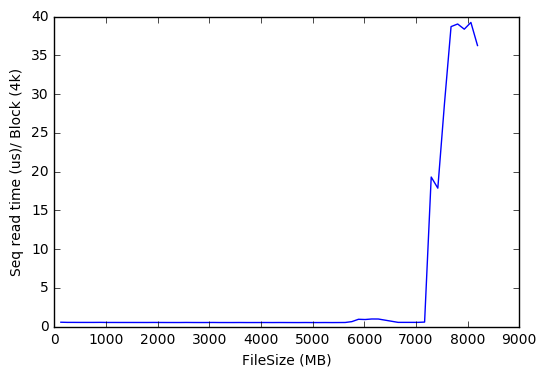
\includegraphics[width = .9\textwidth]{pictures/filecachesize.png}}
    \caption{Reading time of different sized files}
    \label{file_cache_size}
\end{figure}

\textbf{Figure \ref{file_cache_size}} shows how the measured read time varies against different file sizes. We can see that when the file size increases to 7296MB, the reading time increases largely, from 0.5us to 38us. So the file cache size should be about 7296MB (7.1GB), which is in the range we estimated.

\subsection{File Read Time}
\label {File_read_time_section}
\subsubsection{Methodology}
To measure the file read time without file cache, we use the \textbf{open()} system call with the flag \textbf{O_DIRECT}, which indicates reading directly from disk instead of cache. For sequential read time, we use \textbf{read()} to read a 4K block each time and accumulate the total time of reading from offset 0 to the file end. For random read time, we use \textbf{(rand()\%blocknum)*blocksize} to generate read offset and do the sampled read 1000 times for each file. We generate files of sizes from 4MB to 1GB as reading workload. And both the sequential read and random read test are conducted for 10 times and the average read time is calculated as the result

\subsubsection{Estimation and Results}
We estimate the sequential read time would only be determined by the disk data transfer rate, without seek time and rotation latency. So the sequential read time of different sized file would be the same. And since the max data transfer rate is 300Mbps (37.5MB/s), we estimate the sequential read time per block would be:

$$\frac{4KB}{37.5*1000KB/s} = 107us.$$

For the random read time, we take into account seek time and rotation latency. As the rotation speed is 7200RPM, the average rotation latency should be:

$$ \frac{\frac{60s}{7200}}{2} = 4.2ms.$$

And since the usual seek time of a hard disk is about 9ms, the random read time per block should be:
$$ 107us + 4.2ms + 9ms = 13.3ms. $$

And we estimate the random read time will increase as the file size increase, because large files may locates in many cylinders, which requires many head moving while be random read, while small files can be stored in a single cylinder, which requires no head moving.

\begin{figure}[ht]
    \centering
    \frame{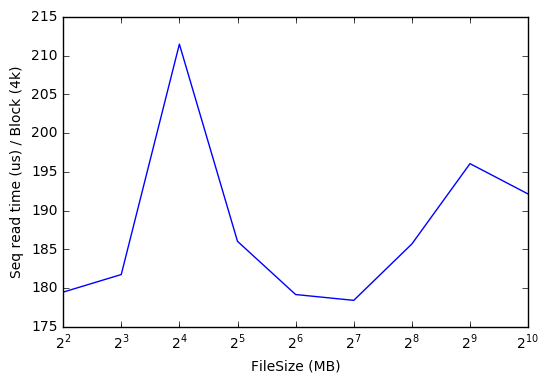
\includegraphics[width = .9\textwidth]{pictures/seqread.png}}
    \caption{Sequential read time per block (4KB)}
    \label{seq_read_time}
\end{figure}

\textbf{Figure \ref{seq_read_time}} shows sequential read time of different file sizes. The total average per-block read time is \textbf{187.8us}, which is a little longer than we estimated (107us). In addition, the read time varies when the file size increase. We speculate the reason is that a file is not totally stored in sequential disk sectors. The data blocks may be on different cylinders, especially for large files. So seeking time and rotation latency are also necessary for
sequential read. And since sequentially reading different-sized files need different times of seeking and rotation, the per-block read time varies. For large files, although more seeking and rotation may be required, but the large block number can also amortize the latency; therefore, a large file may have a shorter read time than a small file, as \textbf{Figure \ref{req_read_time}} shows.


\begin{figure}[ht]
    \centering
    \frame{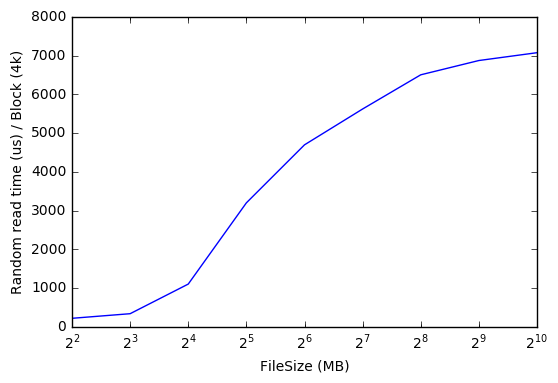
\includegraphics[width = .9\textwidth]{pictures/randread.png}}
    \caption{Random read time per block (4KB)}
    \label{rand_read_time}
\end{figure}

\textbf{Figure \ref{rand_read_time}} shows sequential read time of different file sizes. The average per-block read time increases as the file size increases, as we expected. As aforementioned, the reason is that large files span more sectors and cylinders than small files, so more seeking and rotation is needed for reading. And for small files (4MB to 16MB), increasing of file sizes only causes small increasing of read time, compared to that of large files (16MB to 512MB).
The reason is that file size increasing of small files only leads to more sectors while file size increasing of large files can cause more cylinders.

\subsection{Remote File Read Time}

\subsubsection{Methodology}
To test the read time of remote files, we set up a NFS sever on a different machine, as described in \textbf{Network}, and mount it on our main testing machine. The key challenge is to bypass both the server side and client side file cache. One possible way to address it is use \textbf{O_DIRECT} flag when call open(). However, that flag only take effect when the linux kernel support it, and unfortunately our testing system kernel doesn't support that. As a result,
we adopts another way: free the file cache before conducting test. That is implemented by calling:

\begin{lstlisting}
sudo sh -c 'echo 3>/proc/sys/vm/drop_caches'
\end{lstlisting}

And to avoid NFS transfers more than one block when a data block is read, we set the both read size and write size to 4KB:

\begin{lstlisting}
sudo mount dyn54:/export /mnt -o rsize=4096,wsize=4096
\end{lstlisting}


\subsubsection{Estimation and Results}
We estimate the network penalty with the round trip time and network bandwidth we have measured. \textbf{Section Network} shows that the measured round trip time is 0.338ms (338us) and the peak network bandwidth is 112MB/s, so the network penalty for a block should be:

$$\frac{4KB}{112*1000KB/s} + 338us = 373.7us$$

\begin{figure}[ht]
    \centering
    \frame{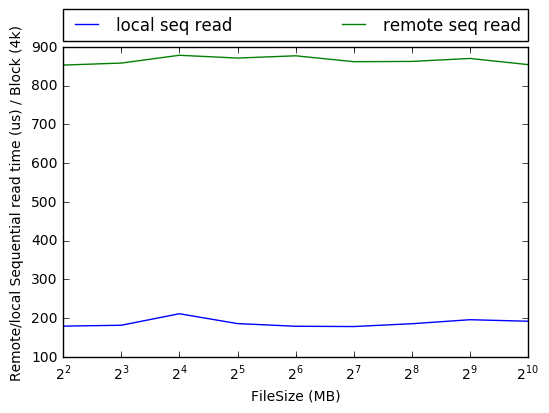
\includegraphics[width = .9\textwidth]{pictures/rseqread.png}}
    \caption{Remote/Local sequential read time per block (4KB)}
    \label{rseq_read_time}
\end{figure}

\textbf{Figure \ref{rseq_read_time}} shows both the remote and local sequential read time of different file sizes. The average per-block read time are 865.3us and 187.8us correspondingly. So the average network penaly is:

$$865.3us - 187.3us = 678us.$$

Compared with our estimated network penalty, the measured one is in the same order of magnitude but almost twice bigger. We speculate the reason is that the NFS implementation introduces additional overhead on read time.

\begin{figure}[ht]
    \centering
    \frame{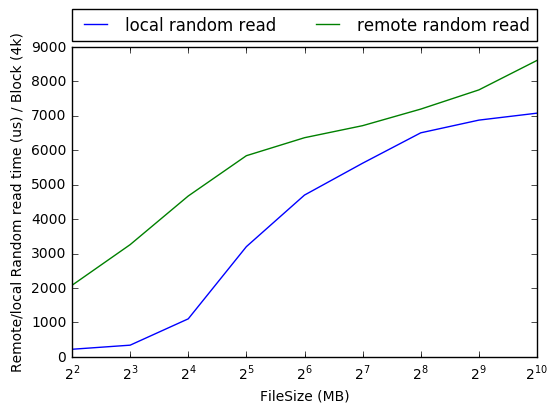
\includegraphics[width = .9\textwidth]{pictures/rrandread.png}}
    \caption{Remote/Local random read time per block (4KB)}
    \label{rrand_read_time}
\end{figure}

\textbf{Figure \ref{rseq_read_time}} shows both the remote and local random read time of different file sizes. The average per-block read time are 4365.2us and 3961.7us correspondingly. So the average network penaly is:

$$5832.3us - 3961.7us = 1870.5us.$$

This penalty is much bigger to the sequential reading one. We speculate the reason is that the remote disk needs more seeking time for random read. The remote disk is 160GB with 8MB cache while local disk is 750GB with 32MB cache. Since the capacity difference, one cylinder of the remote disk should have less sector than the local disk. So the same sized file on the remote disk would span more cylinder than on the local disk, which leads to more seeking time.

\subsection{Contention}
\subsubsection{Methodology}
To measure the contention effect of different process reading different files on the same disk, we generate \textbf{10} different files with the same size of \textbf{128MB} and create \textbf{1} to \textbf{10} processes to do the reading test. We uses the \textbf{open()} call with \textbf{O_DIRECT} to bypass the file cache, same as \textbf{Section \ref{File_read_time_section}}. To calculate the time of reading a block, we write test program to sequentially read the file once a block from the beginning to the end and calculate the average time as the result. We repeat the each test for 10 times to eliminate outerliers.

\subsubsection{Estimation and Results}
Since different processes share the same disk bandwidth when they read the same disk simultaneously, we estimate the reading time increases by times of the process number. As we measured before, the per-block read time of one process is 188us, we estimate contented read time would be:
$$process number * 188us$$

\begin{figure}[ht]
    \centering
    \frame{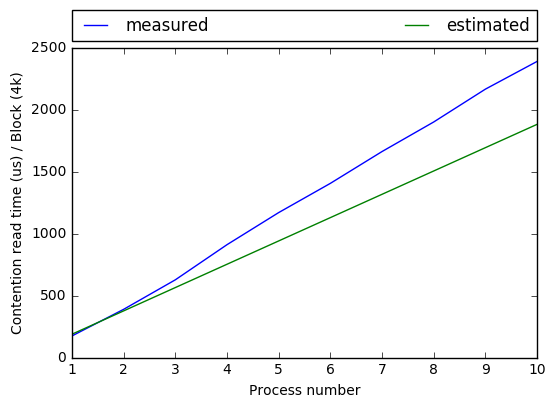
\includegraphics[width = .9\textwidth]{pictures/contention.png}}
    \caption{Remote/Local random read time per block (4KB)}
    \label{contention_read_time}
\end{figure}

\textbf{Figure \ref{contention_read_time}} show the per-block read time with contention of different process number. We can see that the measured read time increase linearly almost as the line:
$$ read time = 174 + process * 240 (us)$$
The measured read time is quite close to our estimation but a little bit higer. That is reasonable since we have not taken into account the process switch overhead.


\end{document}
